% ****** Start of file apssamp.tex ******
%
%   This file is part of the APS files in the REVTeX 4.1 distribution.
%   Version 4.1r of REVTeX, August 2010
%
%   Copyright (c) 2009, 2010 The American Physical Society.
%
%   See the REVTeX 4 README file for restrictions and more information.
%
% TeX'ing this file requires that you have AMS-LaTeX 2.0 installed
% as well as the rest of the prerequisites for REVTeX 4.1
%
% See the REVTeX 4 README file
% It also requires running BibTeX. The commands are as follows:
%
%  1)  latex apssamp.tex
%  2)  bibtex apssamp
%  3)  latex apssamp.tex
%  4)  latex apssamp.tex
%
\documentclass[%
 reprint,
%superscriptaddress,
%groupedaddress,
%unsortedaddress,
%runinaddress,
%frontmatterverbose, 
%preprint,
%showpacs,preprintnumbers,
%nofootinbib,
%nobibnotes,
%bibnotes,
 amsmath,amssymb,
 aps,
%pra,
prb,
%rmp,
%prstab,
%prstper,
floatfix,
]{revtex4-1}

\usepackage{graphicx}% Include figure files
\usepackage{dcolumn}% Align table columns on decimal point
\usepackage{bm}% bold math
\usepackage[colorlinks=true, citecolor=red, linkcolor=blue, urlcolor=black]{hyperref}% add hypertext capabilities
%\usepackage[mathlines]{lineno}% Enable numbering of text and display math
%\linenumbers\relax % Commence numbering lines

%\usepackage[showframe,%Uncomment any one of the following lines to test 
%%scale=0.7, marginratio={1:1, 2:3}, ignoreall,% default settings
%%text={7in,10in},centering,
%%margin=1.5in,
%%total={6.5in,8.75in}, top=1.2in, left=0.9in, includefoot,
%%height=10in,a5paper,hmargin={3cm,0.8in},
%]{geometry}

\usepackage{enumerate}
\usepackage{subfig}

\def\d{{\textit{d}}}
\newcommand*{\field}[1]{\mathbb{#1}}%

\newcommand{\bra}[1]{\langle#1\rvert}
\newcommand{\ket}[1]{\lvert#1\rangle}
\newcommand{\mean}[1]{\langle#1\rangle}

\newcommand{\Bra}[1]{\left\langle#1\left\rvert}
\newcommand{\Ket}[1]{\right\lvert#1\right\rangle}

\newcommand{\K}{\operatornamewithlimits{\mathcal{K}}}

\def\tj{{$t$--$J$}}
\def\tjz{{$t$--$J^z$}}
\def\square{{$\mathbb{Z}^2$}}

% %%%%%%
% pkgs to be removed in the final version:
\usepackage[dvipsnames]{xcolor}
\usepackage[normalem]{ulem}
\usepackage{ifthen}

\newcounter{verbosity}
\setcounter{verbosity}{1}
% verbosity = 0 -> only important comments
% verbosity = 1 -> all comments
% %%%%%

\begin{document}

%\preprint{APS/123-QED}


\title{Title?}

%\title{Magnon-magnon Interaction Induced Incoherence in the 2D  Doped Antiferromagnets}% Force line breaks with \\
%\thanks{A footnote to the article title}%

\author{Adam K\l{}osi\'n{}ski$^1$}
\author{Piotr Wrzosek$^1$}
\author{Cli\`o{} Agrapidis$^{1,2}$}
\author{Krzysztof Wohlfeld$^1$}
 
\affiliation{%
$^1$Institute of Theoretical Physics, Faculty of Physics, University of Warsaw, Pasteura 5, PL-02093 Warsaw, Poland
}%


\date{\today}% It is always \today, today,
             %  but any date may be explicitly specified

\begin{abstract}
Here goes the abstract...

\end{abstract}

\pacs{Valid PACS appear here}% PACS, the Physics and Astronomy
                             % Classification Scheme.
%\keywords{Suggested keywords}%Use showkeys class option if keyword
                              %display desired
\maketitle

%\tableofcontents

\section{\label{sec:intro}Introduction}

\section{Model}

We consider the following model on the Bethe lattice
\begin{equation}\label{model}
\begin{aligned}
\mathcal{H} = -t &\sum_{\mean{i,j}} \left[ h_i^\dag h_j \left(a_i + a_j^\dag (1 - a_i^\dag a_i) \right)\right. + \\
&+ \left. h_j^\dag h_i \left(a_j + a_i^\dag (1 - a_j^\dag a_j) \right)\right] + \sum_i J_i a_i^\dag a_i,
\end{aligned}
\end{equation}
describing hopping of a hole $(h_i)$ on the lattice accompanied by creation or annihilation of magnons $(a_i)$. We calculate the spectral function,
\begin{equation}
A(\omega) = -\frac{1}{\pi}\text{Im}\!\left(G(\omega + i0^+)\right)
\end{equation}
of a single hole in such system. States with both hole and the magnon at the same site are projected out $(1 - a_i^\dag a_i)$. In general, the model describes the problem of a particle travelling through the lattice and exciting/relaxing the lattice by an amount of energy dependent on the position of the particle. 

\subsection{Relation to the $t\text{-}J^z$~model}
 
For constant $J_i \propto J$ the above model is an approximation of the $t\text{-}J^z$~model with a single hole,
\begin{equation}
\mathcal{H}_{t\text{-}J^z} = -t \sum_{\mean{i,j},\sigma} \left(
\tilde{c}_{i\sigma}^{\dag}\tilde{c}_{j\sigma}^{}\!+\!\mathrm{H.c.}\!\right)
+ J \sum_{\mean{i,j}}\left( S_{i}^{z}S_{j}^{z}\!
-\tfrac14\,\tilde{n}_i\tilde{n}_j\right),
\end{equation}
expressed in terms of hole and magnon operators with potential energy proportional to $J$ treated within the linear spin wave (LSW) theory. The transformation starts with the rotation of spins on one sublattice
\begin{equation}
\mathcal{H}_{\text{rot}} = -t \sum_{\mean{i,j},\sigma} \left( \tilde{c}_{i\sigma}^\dag \tilde{c}_{j\bar{\sigma}} + \text{H.c.} \right) - J \sum_{\mean{i,j}} ( S_i^z S_j^z + \frac{1}{4} \tilde{n}_i \tilde{n}_j ).
\end{equation}
It allows for introduction of holes and magnons in terms of following transformations,
\begin{equation}
\begin{aligned}
\tilde{c}_{i\uparrow}^\dag &= h_i, &\quad \tilde{c}_{i\uparrow} &= h_i^\dag (1 - a_i^\dag a_i), \\
\tilde{c}_{i\downarrow}^\dag &= h_i a_i^\dag, &\quad \tilde{c}_{i\downarrow} &= h_i^\dag a_i,
\end{aligned}
\end{equation}
\begin{equation}
\begin{aligned}
S_i^z &= \frac{1}{2} - a_i^\dag a_i - \frac{1}{2}h_i^\dag h_i, \\
\tilde{n}_i &= 1 - h_i^\dag h_i.
\end{aligned}
\end{equation}
Then, kinetic energy in terms of hole and magnon operators reads,
\begin{equation}
\begin{aligned}
\mathcal{H}_t = -t \sum_{\mean{i,j}} &\left[ h_i^\dag h_j \left( a_i + a_j^\dag (1 -  a_i^\dag a_i) \right)\right. + \\
&+ \left. h_j^\dag h_i \left( a_j + a_i^\dag (1 -  a_j^\dag a_j) \right)\right].
\end{aligned}
\end{equation}
Accordingly, the potential energy reads,
\begin{equation}
\begin{aligned}
\mathcal{H}_J &= E_0 + \frac{J}{2} \sum_{\mean{i,j}} \left[ a_i^\dag a_i + a_j^\dag a_j - 2 a_i^\dag a_i a_j^\dag a_j \right. + \\
&+\left. h_i^\dag h_i + h_j^\dag h_j - h_i^\dag h_i a_j^\dag a_j - h_j^\dag h_j a_i^\dag a_i - h_i^\dag h_i h_j^\dag h_j \right].
\end{aligned}
\end{equation}
Neglecting constant energy shift, magnon-magnon interactions (LSW) and terms related to the holes (which do not play qualitative role assuming there is a single hole in the system) one ends up with the model stated in Eq. \ref{model} with $J_i$ constant.

\section{Bethe Lattice}
\subsection{Methods}

In a case of the Bethe lattice with coordination number $z$ one can obtain a convenient basis of states reachable from initial state $\ket{0}$, that tridiagonalizes the matrix of the model Hamiltonian in the reachable subspace. The initial state $\ket{0}$ is a state without magnons with a single hole located at the origin, i.e. at site $i = 0$. The number of possible states that can be achieved with a single hop of a hole is equal to the coordination number $z$, so there are $z$ reachable states with one magnon. We denote the normalized sum of those as $\ket{1}$. Similarly, there are $z(z-1)$ states with 2 magnons. The factor $z-1$ comes from the fact that once hole leaves the origin then one site in the proximity of a hole is occupied by a magnon. Normalised sum of reachable states with 2 magnons is denoted as $\ket{2}$. For $n > 0$ there are $z(z-1)^{n-1}$ reachable states with normalised sum denoted as $\ket{n}$. In basis $\mathcal{B} = (\ket{0}, \ket{1}, \ket{2}, ...)$ the matrix of the Hamiltonian appears tridiagonal,
\begin{equation}
\mathcal{M}(\mathcal{H})=\begin{bmatrix}
V_0 & -t\sqrt{z} &  &  &  \\
-t\sqrt{z} & V_1 & -t\sqrt{z-1} &  &  \\
 & -t\sqrt{z-1} & V_2 & -t\sqrt{z-1}&  \\
 &  &  -t\sqrt{z-1} & V_4 & \ddots \\
 &  &  & \ddots & \ddots \\
\end{bmatrix},
\end{equation}
where $V_i = \sum_{k=0}^{i-1} J_k$. This yields a simple formula for the Greens function in a form of a continued fraction,
\begin{equation}
G(\omega) = \left\langle 0 \left| \frac{1}{\omega - \mathcal{H}} \right| 0 \right\rangle \\
= \frac{1}{\omega - V_0 - \Sigma(\omega)},
\end{equation} 
where the corresponding expression for self-energy appears as follows,
\begin{equation}
\Sigma(\omega) = \frac{zt^2}{\omega - V_1 - \frac{(z-1)t^2}{\omega - V_2 - \hdots}}.
\end{equation}

\subsection{Point Potential Results}

In particular, we study the problem of a single hole on the Bethe lattice in the case of a point potential located at the origin (i.e. in the position where the hole was created in the system). It corresponds to $J_i = V$, when $i = 0$ and $J_i = 0$ otherwise. This leads to the following expression for the self-energy,
\begin{equation}
\begin{aligned}
&\Sigma(\omega) = \frac{zt}{z-1} \left( \frac{\omega - V}{2t} \pm \sqrt{\left( \frac{\omega - V}{2t} \right)^2 - (z-1)} \right).
\end{aligned}
\end{equation}
From the above on can easily calculate the analytic formula for the quasiparticle residue $z_0$ and the limiting value $V^*$ for which the system undergoes transition form having to not having quasiparticle solution. 
\begin{equation}
\begin{aligned}
z_0&(z,t,V) = \lim_{\omega\to\omega^*}(\omega - \omega^*)G(\omega) = \lim_{\omega\to\omega^*}\frac{1}{1-\frac{d}{d\omega}\Sigma(\omega)} \\ 
&= \left( \frac{z-2}{2(z-1)} + \frac{1}{\sqrt{1 - \frac{16t^2(z-1)}{ \left( (z-2)V-z\sqrt{V^2 + 4t^2} \right)^2}}}  \right)^{-1},
\end{aligned}
\end{equation}
\begin{equation}
V^*(z,t) = t\frac{z-2}{\sqrt{z-1}}.
\end{equation}

\begin{figure}[ht!]
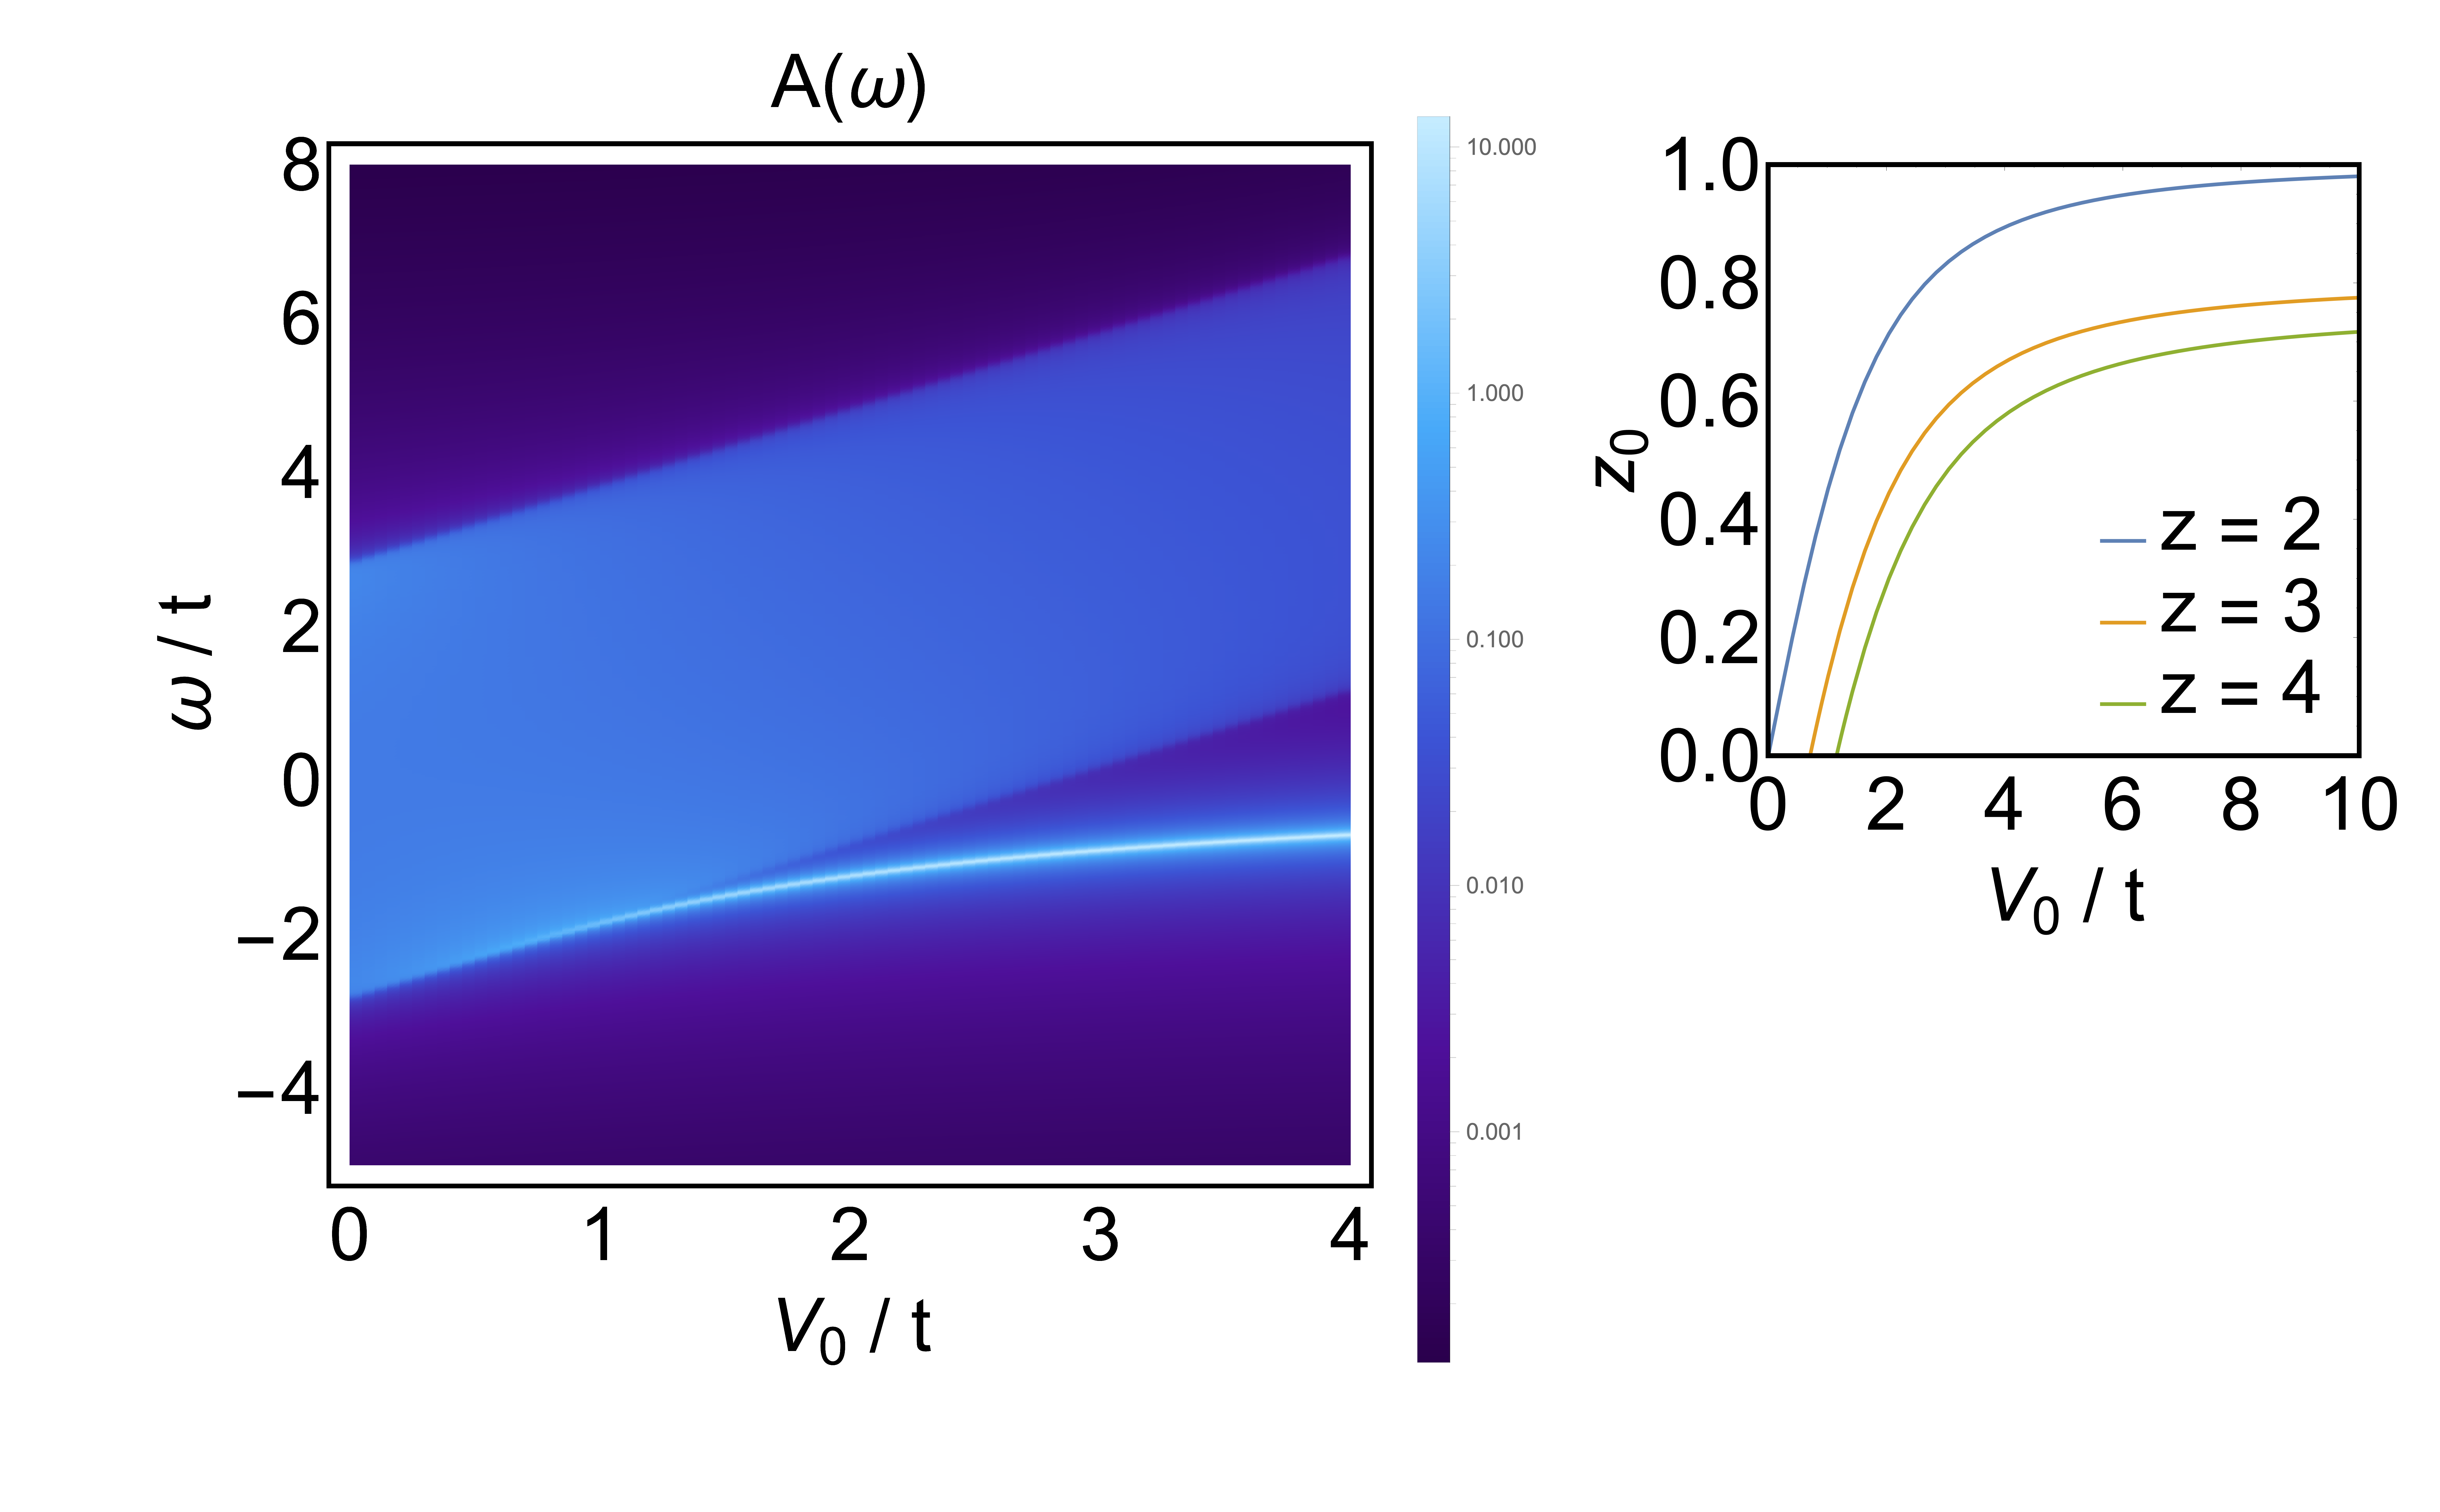
\includegraphics[width=0.45\textwidth]{plot1}
\caption{Spectral function of a single hole for various strengths of a point potential $V_0$ and coordination number $z = 3$ (left) and quasiparticle residue $z_0(V_0)$ for few coordination numbers $z$ (right). In the figure of the spectral function (left) the transition occurs at $V_0 = \frac{t}{\sqrt{2}} \approx 0.7t$.}
\label{pointpotential}
\end{figure}

\subsection{Arbitrary Potential Shape}

Let us consider more general case. Now we take arbitrary shape of the on site potential $V_k$, where $k$ stands for the distance from the origin. Let us denote $\Gamma(\omega) = \frac{(z-1)t^2}{\omega - V - \Gamma(\omega)}$, $\Omega_k = \omega - V_{k<n}$, $\Omega_n = \frac{(z-1)t^2}{\Gamma(\omega)}$, $\tau_1 = zt^2$ and $\tau_{k>1} = (z-1)t^2$. Then we can write down the expression for the self-energy as follows,
\begin{equation}
\begin{aligned}
\Sigma(\omega) = \frac{\tau_1}{\Omega_1 - \frac{\tau_2}{\Omega_2 - \frac{\tau_3}{\Omega_3 - \hdots}}} = \frac{z}{z-1}\K_{k=1}^n \left(\frac{\tau_2}{\Omega_k}\right).
\end{aligned}
\end{equation}
In order to obtain the expression for the quasi-particle residue 
\begin{equation}
z_0 = \lim_{\omega\to\omega^*}\frac{1}{1-\frac{d}{d\omega}\Sigma(\omega)},
\end{equation}
we calculate the derivative of the self-energy with respect to frequency $\omega$,
\begin{equation}
\begin{aligned}
\frac{d}{d\omega} \Sigma(\omega) &= \frac{z}{z-1} \frac{d}{d\omega} \K_{k=1}^n \left(\frac{\tau_2}{\Omega_k}\right) = \\
&= \frac{z}{(z-1)^2t^2}\sum_{j=1}^n \left(-1 \right)^{j+1} \prod_{k=1}^j \left[ \K_{l=k}^n \left(\frac{\tau_2}{\Omega_l}\right) \right]^2 \frac{d\Omega_j}{d\omega},
\end{aligned}
\end{equation}
where $\frac{d}{d\omega}\Omega_{j<n} = 1$ and $\frac{d}{d\omega}\Omega_n = \frac{d}{d\omega}\left( \frac{(z-1)t^2}{\Gamma(\omega)} \right)$. Note, $V^*$ is not well defined in general, so we do not provide any expression here.
~~
\begin{figure}[ht!]
\centering
\includegraphics[width=0.45\textwidth]{anypot}
\caption{Shape of the potential $V_k$ confining the hole (left) and the spectral function of a single hole (right) for $J_{k \in \{0,1,2\}} = (\frac{3}{2}-\frac{k}{2})t$ and $J_{k>2} = 0$. Coordination number $z = 3$. The quasiparticle solution is well separated from the continuum.}
\end{figure}

\newpage
\subsection{Linear Potentials}

In what follows we investigate properties of the spectral function of a single hole for linearly shaped potentials. Further analysis includes four cases:
\begin{enumerate}[(i)]
\item constant area enclosed by the linear potential well with the width of the well changing (Fig. \ref{areaconst}),
\item constant depth of the well with the width varying (Fig. \ref{V0const}),
\item constant width with varying depth (Fig. \ref{widthconst}),
\item constant slope of the well for various width of the well (Fig. \ref{stepconst}).
\end{enumerate}

\begin{figure}[ht!]
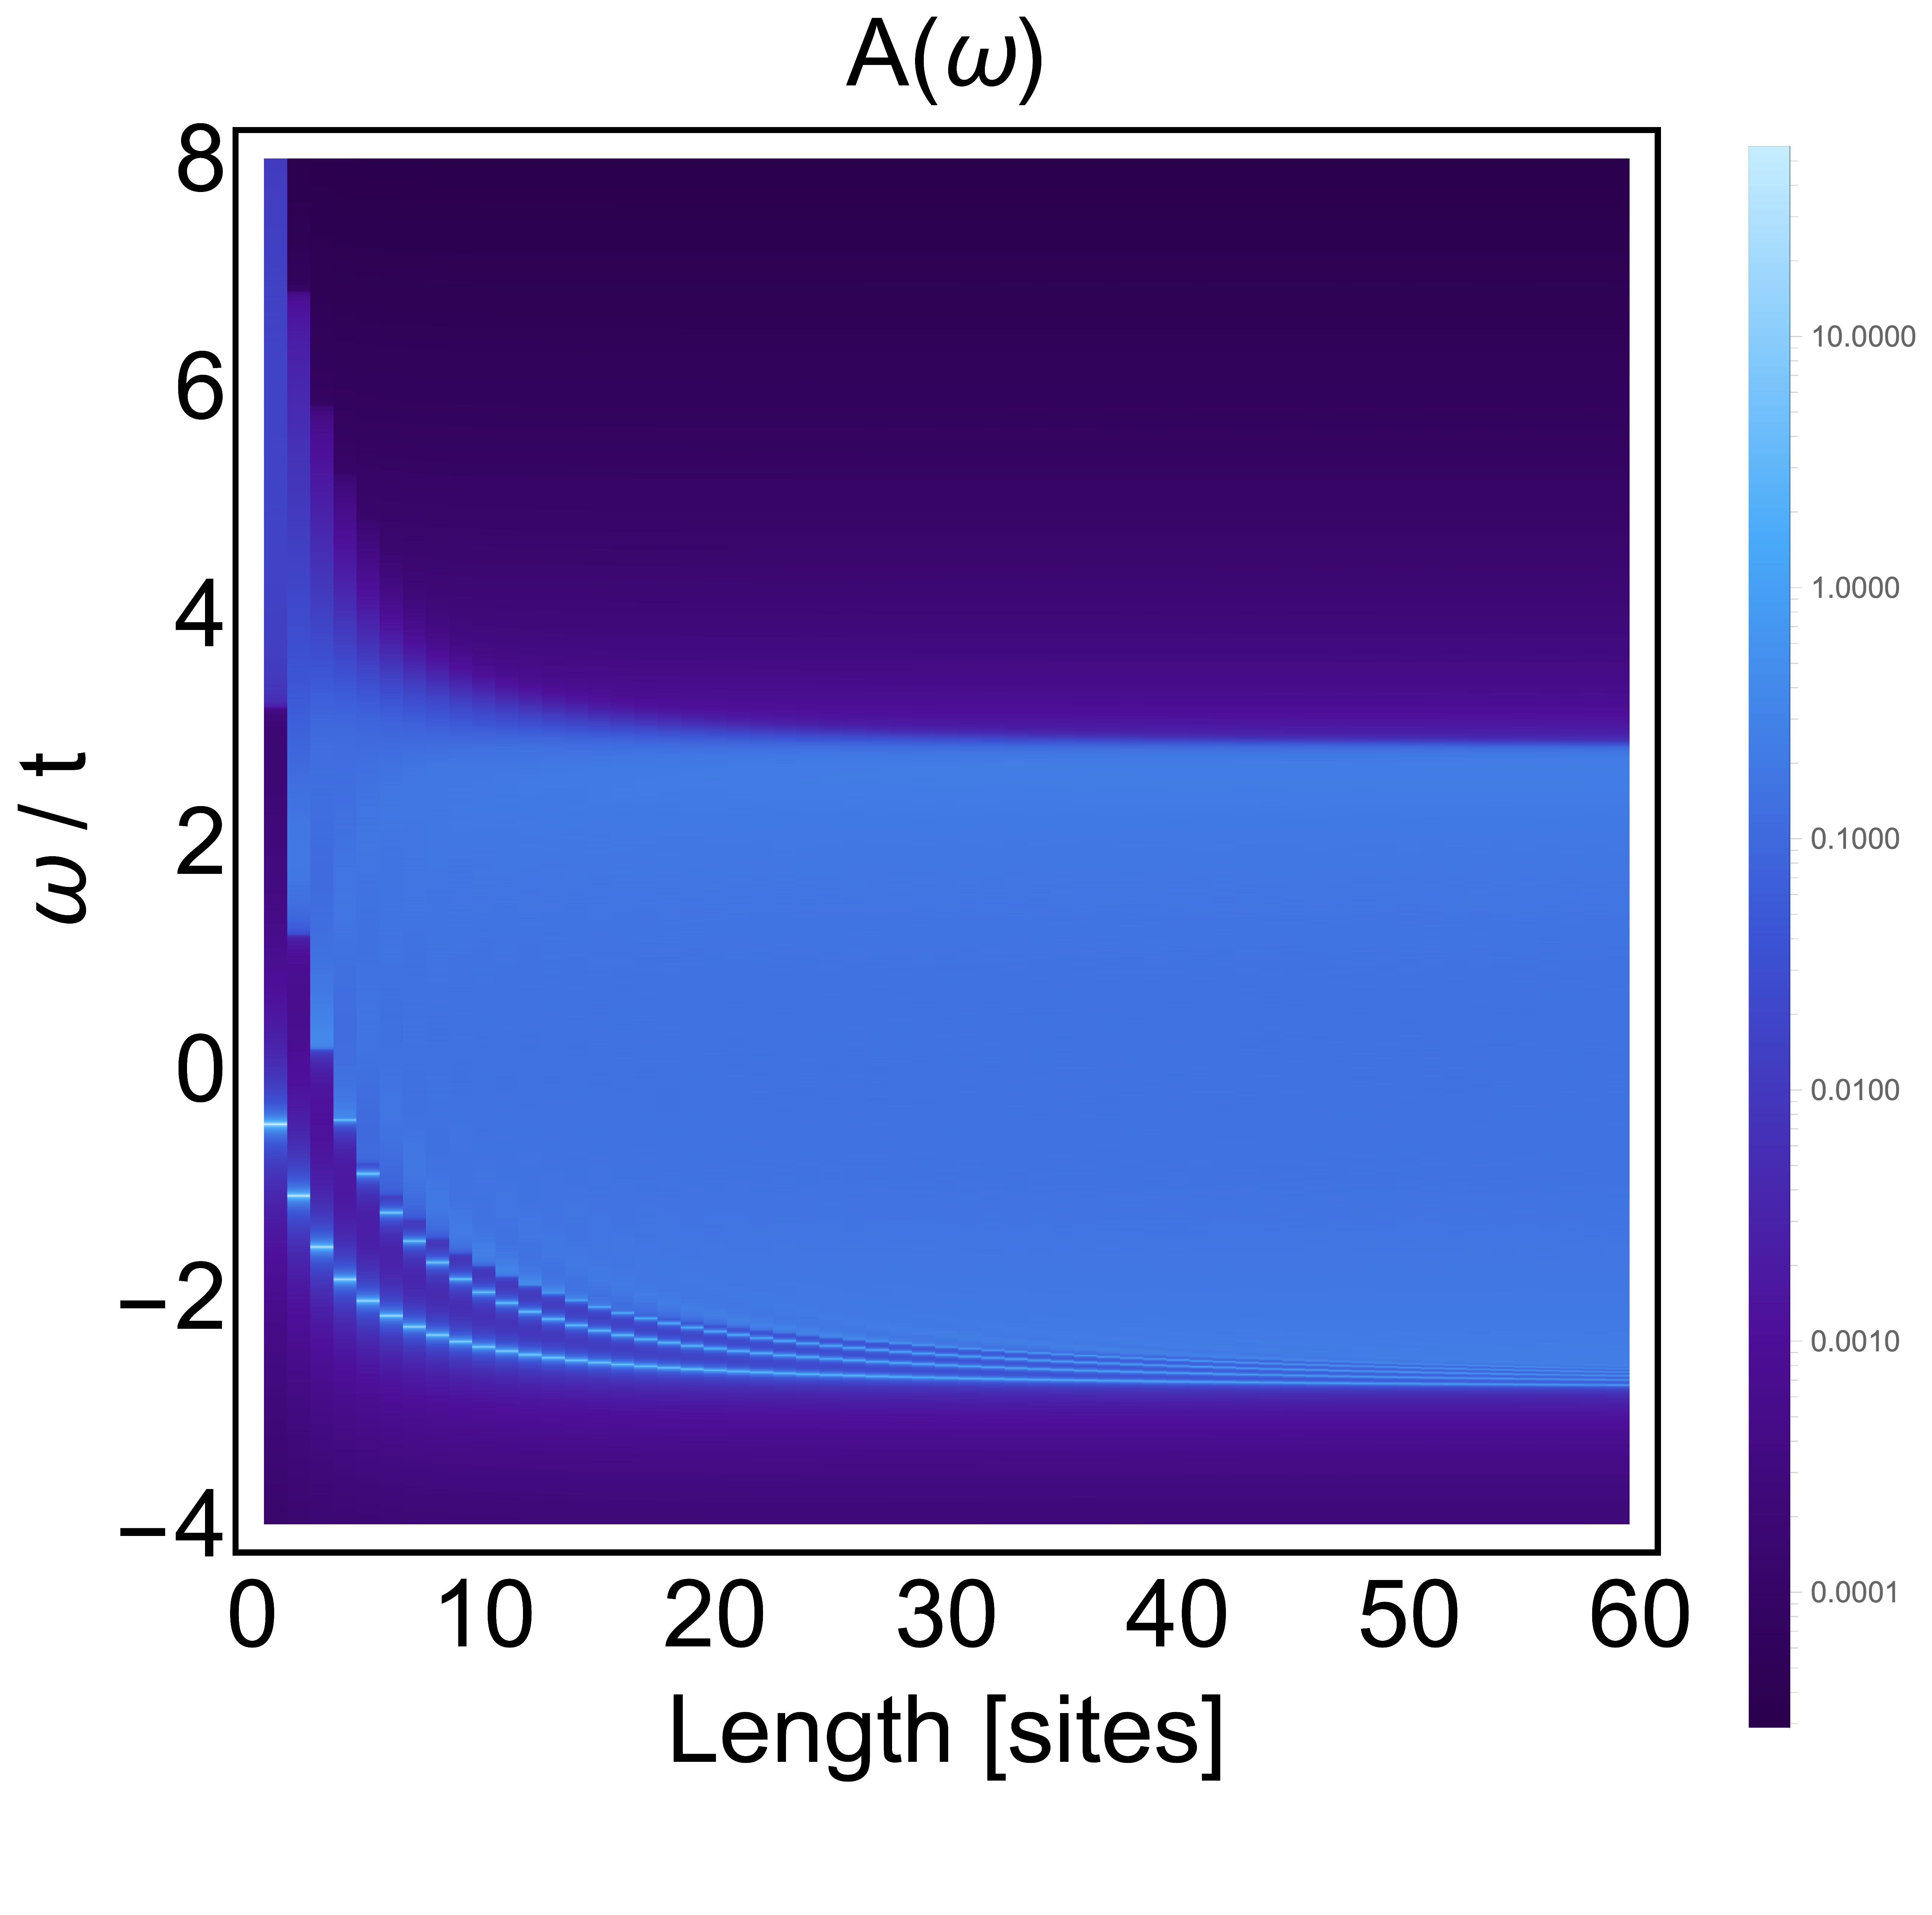
\includegraphics[width=0.4\textwidth]{areaconst}
\caption{Spectral function of a single hole for constant `area' of the potential $A = 6t$. Coordination number $z = 3$. Transition from single quasiparticle (through multiple QPs) into a continuum is observed.}\label{areaconst}
\end{figure}

\begin{figure}[ht!]
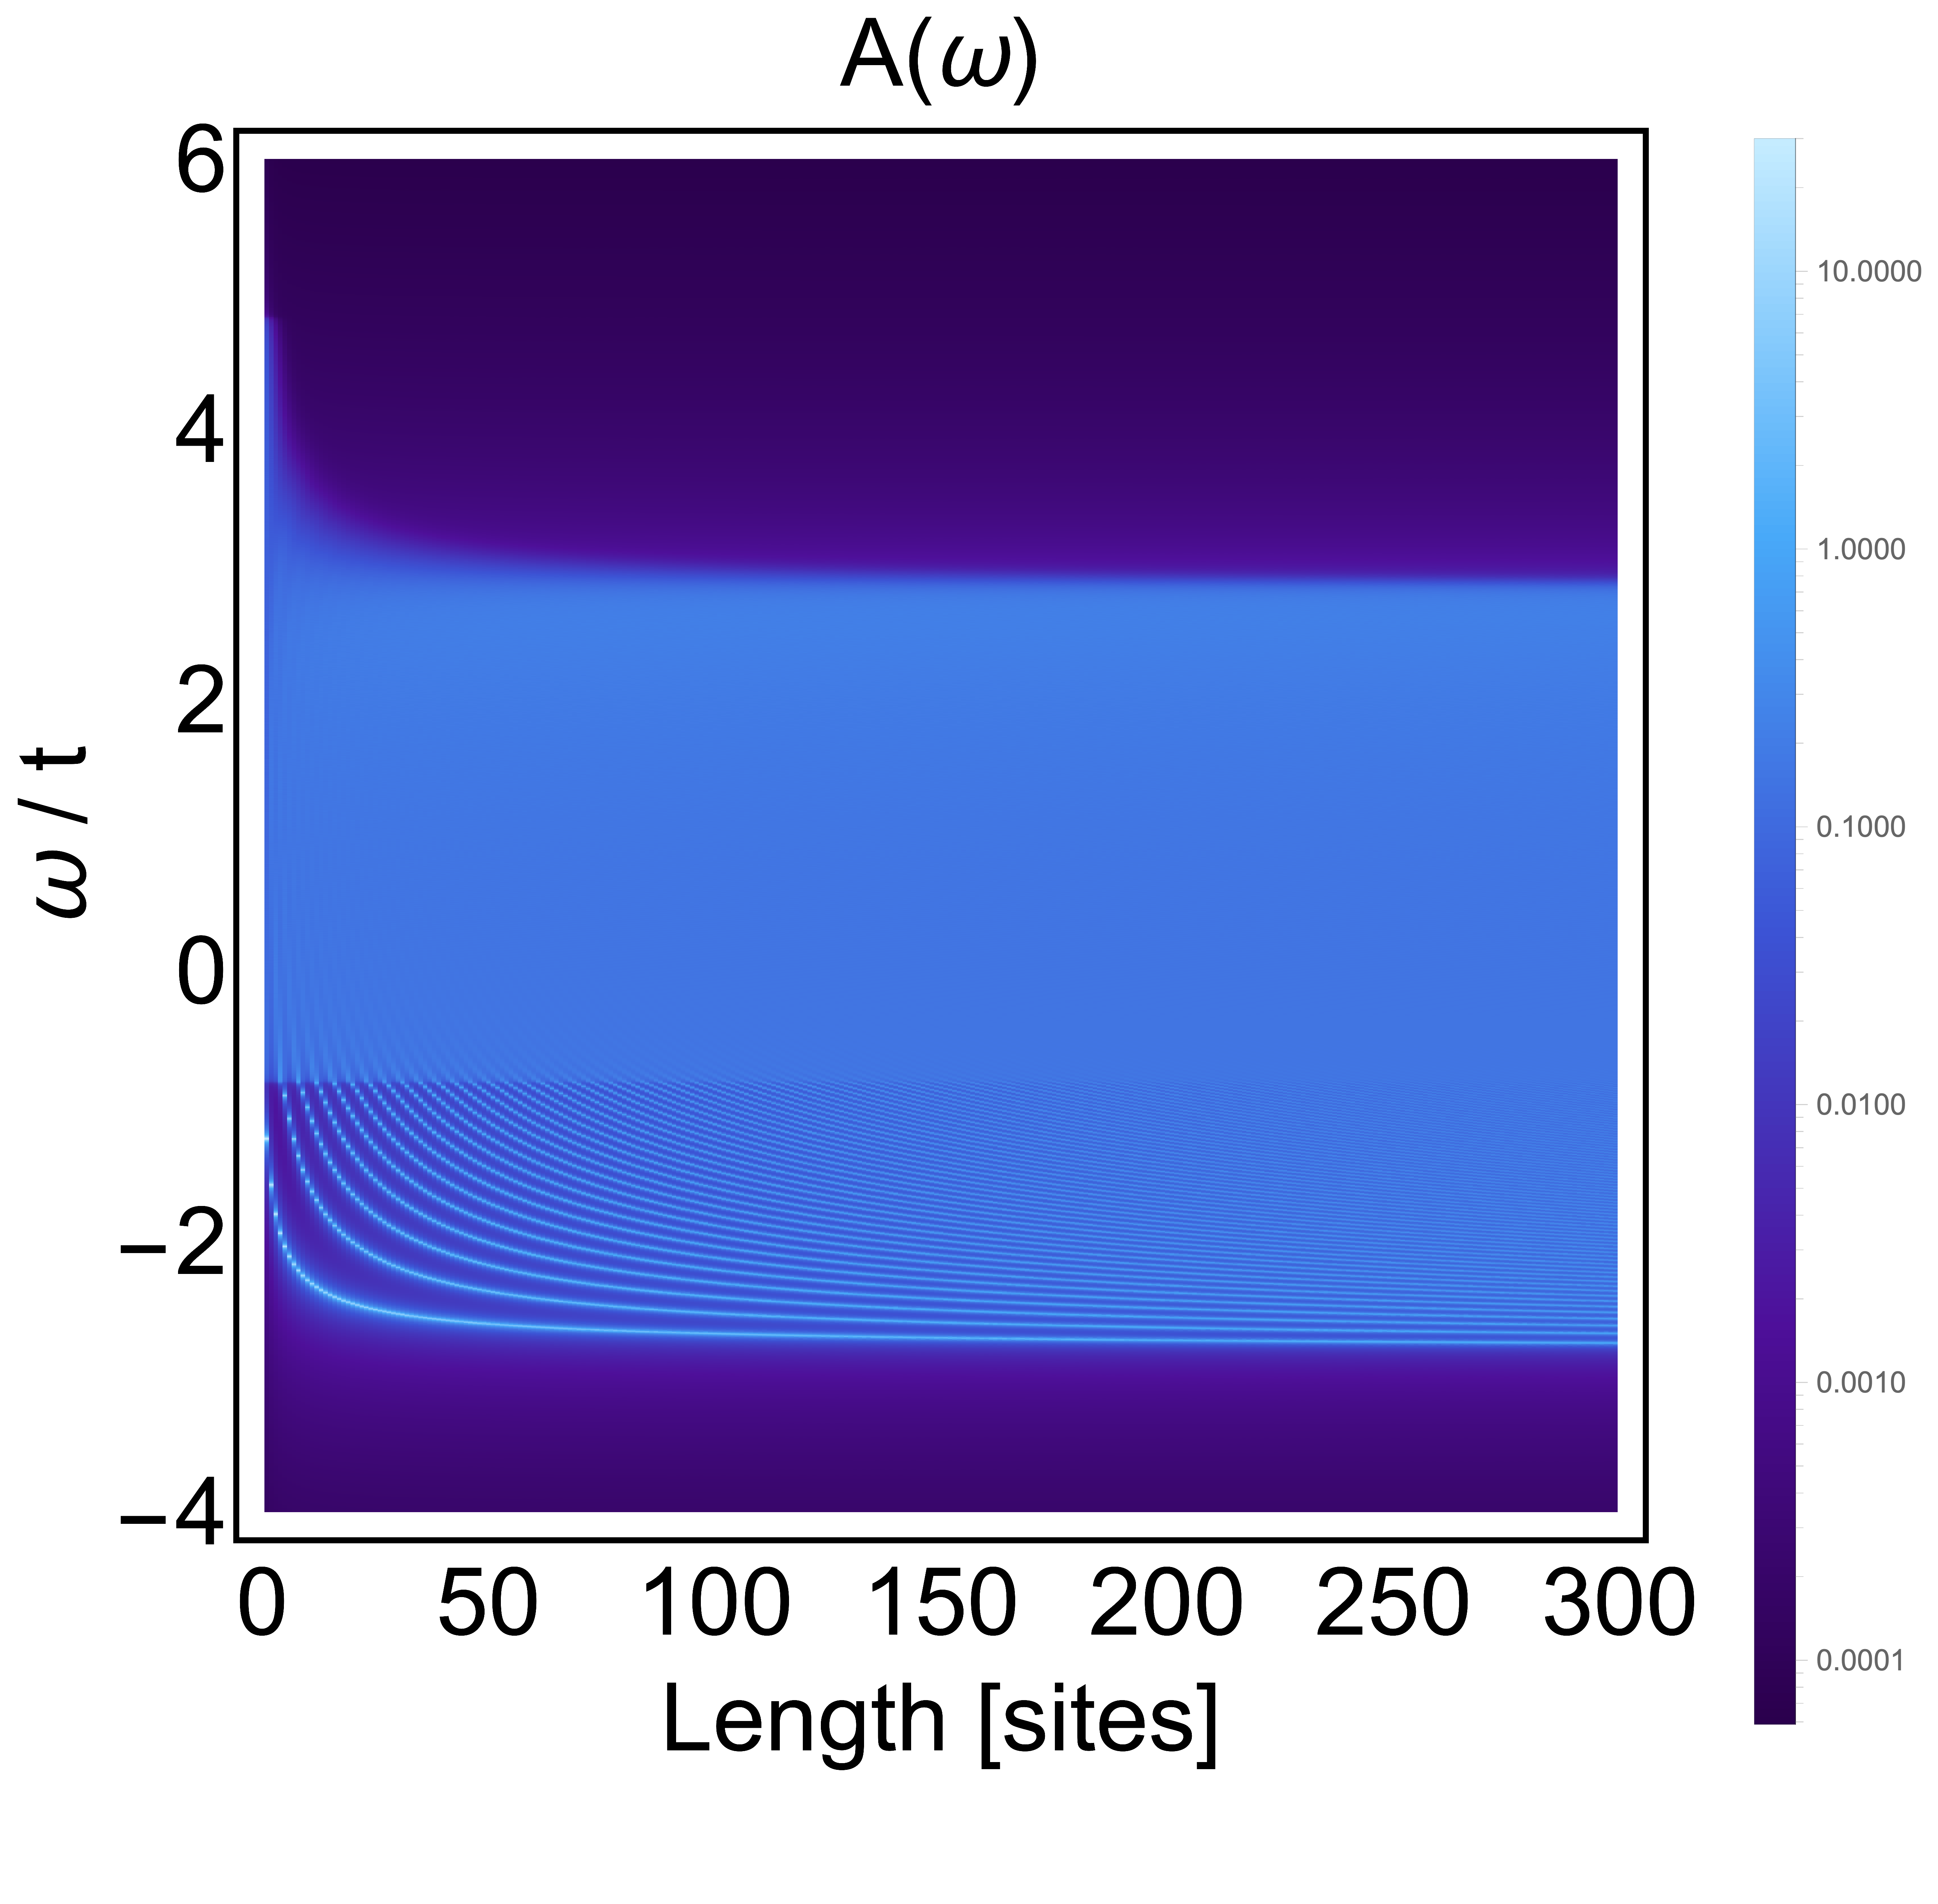
\includegraphics[width=0.4\textwidth]{V0const}
    \caption{Spectral function of a single hole for constant potential depth $V_0 = 2t$. Coordination number $z = 3$. Dependent on the $V_0$ transition from no QP to single QP and then through multiple QPs into a continuum can be observed.}\label{V0const}
\end{figure}

\begin{figure}[ht!]
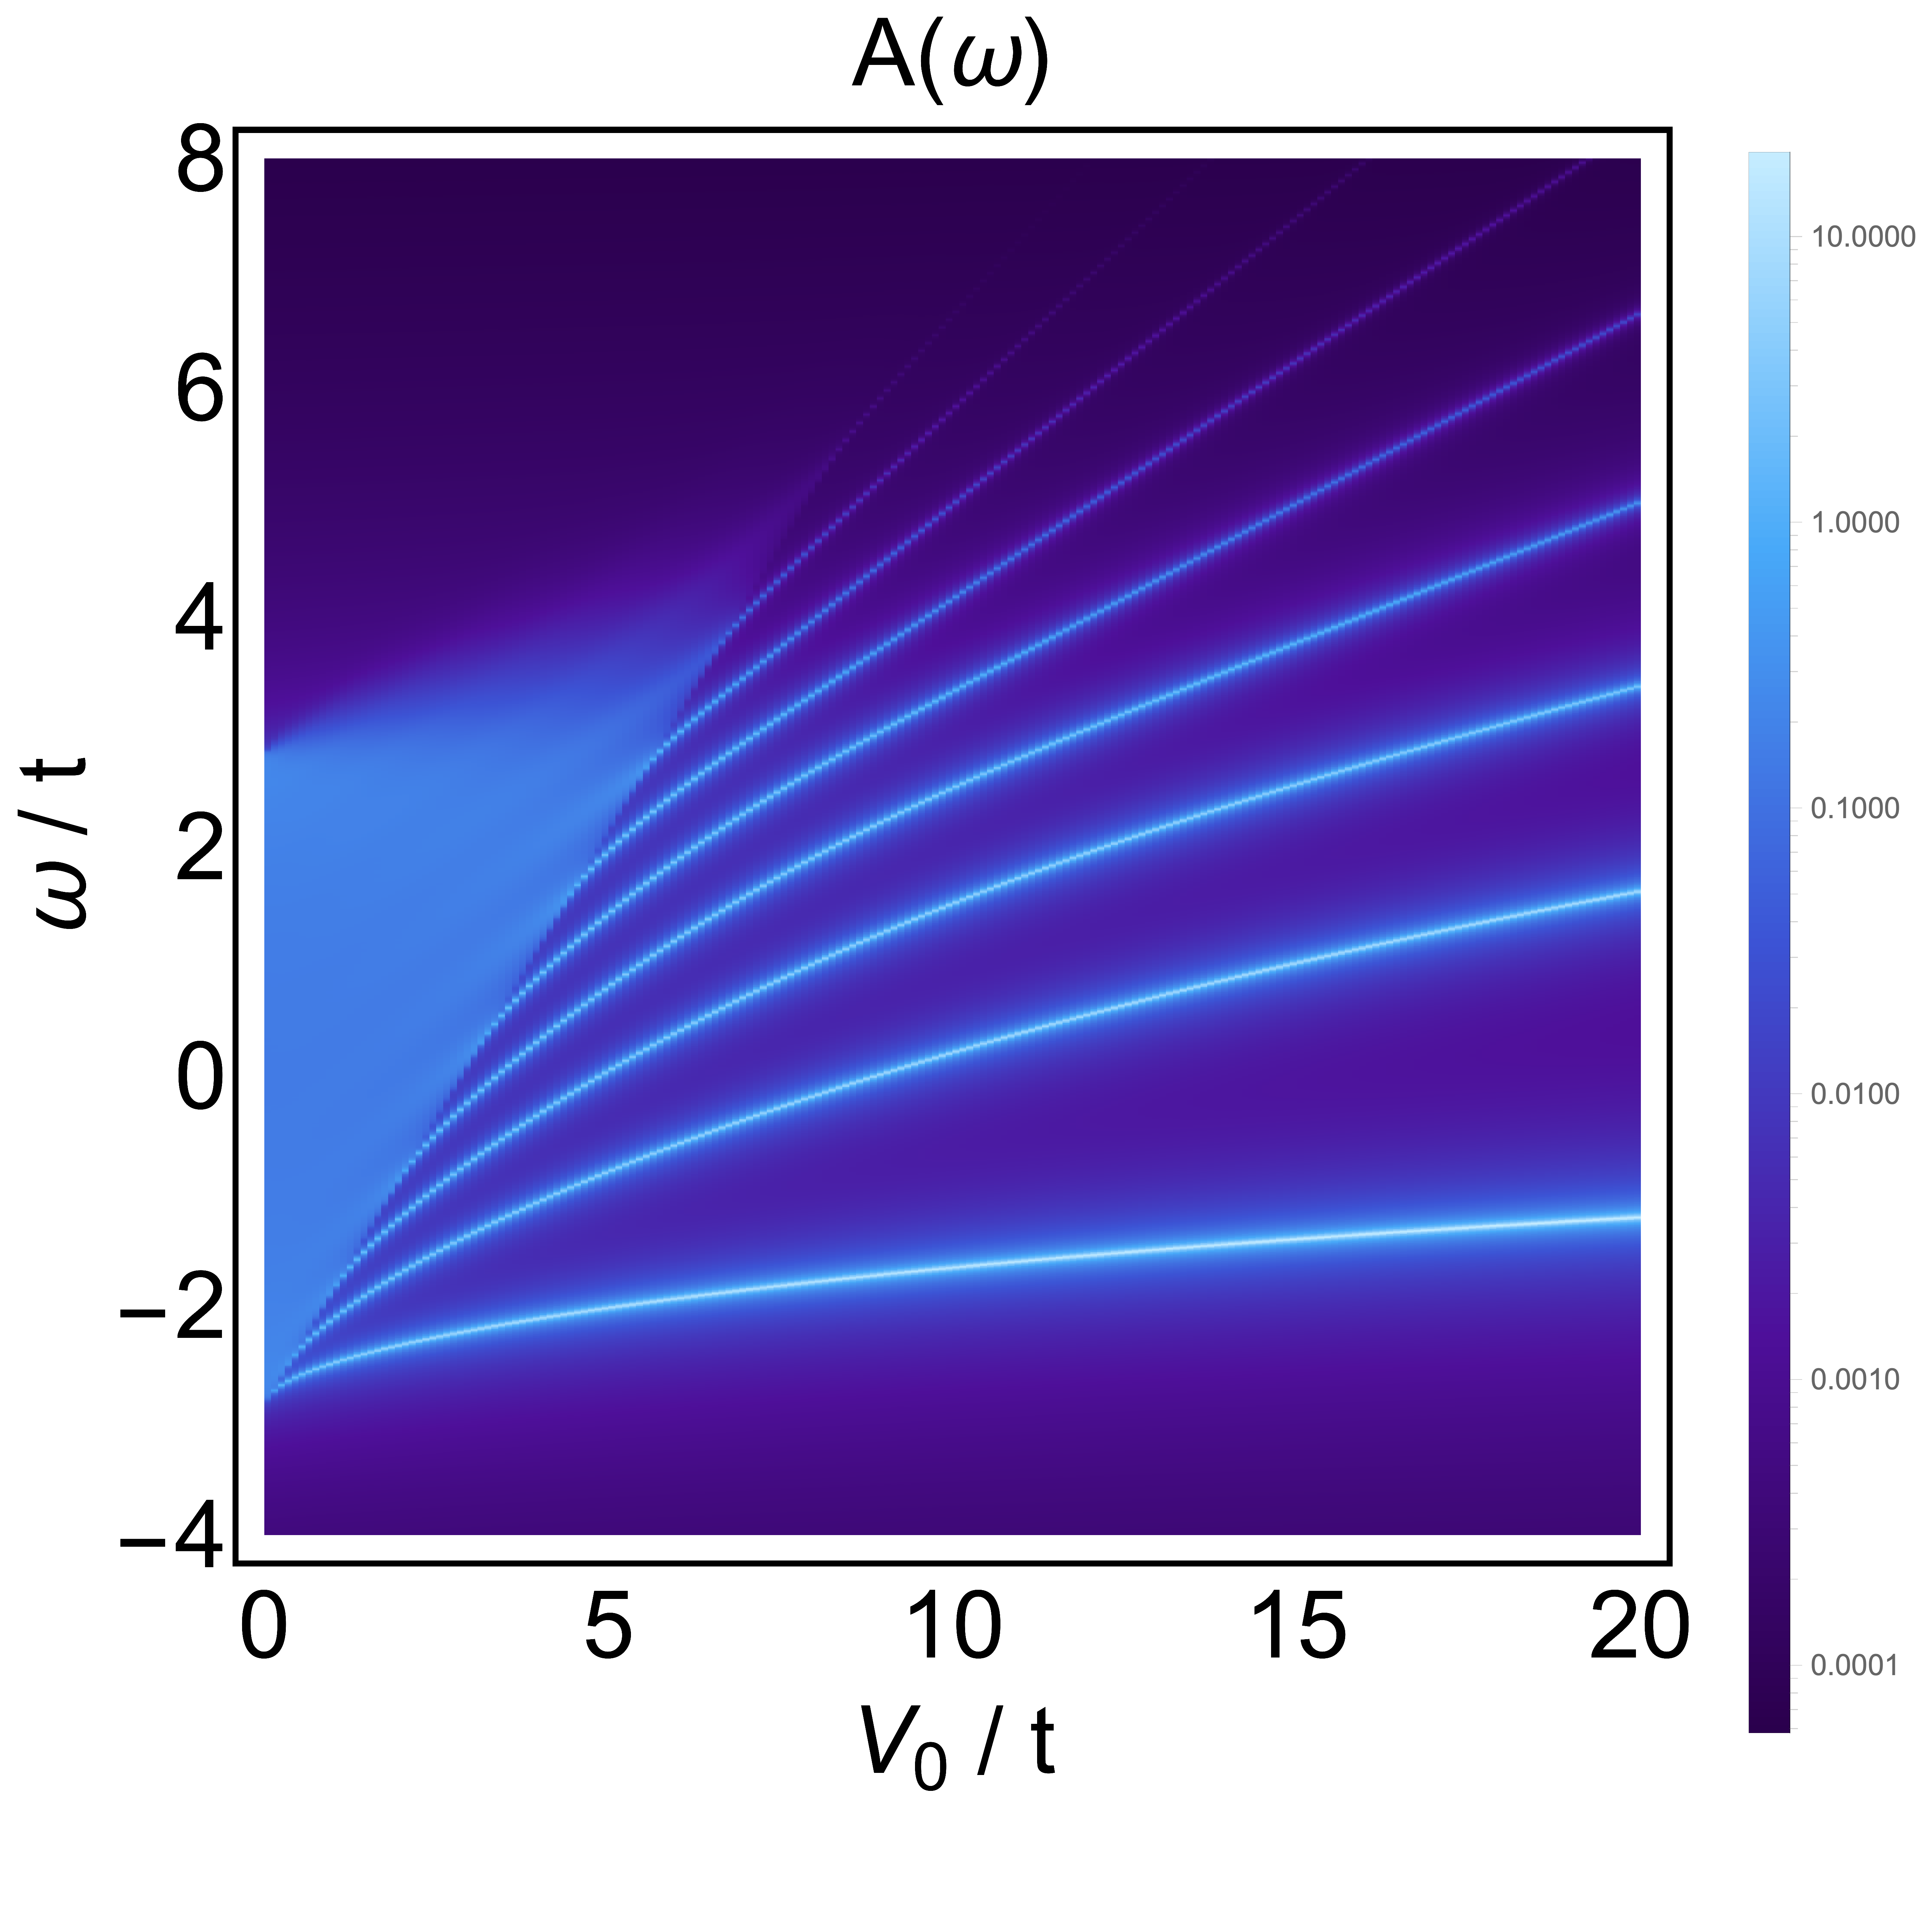
\includegraphics[width=0.4\textwidth]{Widthconst}
    \caption{(Spectral function of a single hole for constant `half-width' of the well $L = 12$ sites. Coordination number $z = 3$. Transition from continuum into a multiple QPs is observed.}\label{widthconst}
\end{figure}

\begin{figure}[ht!]
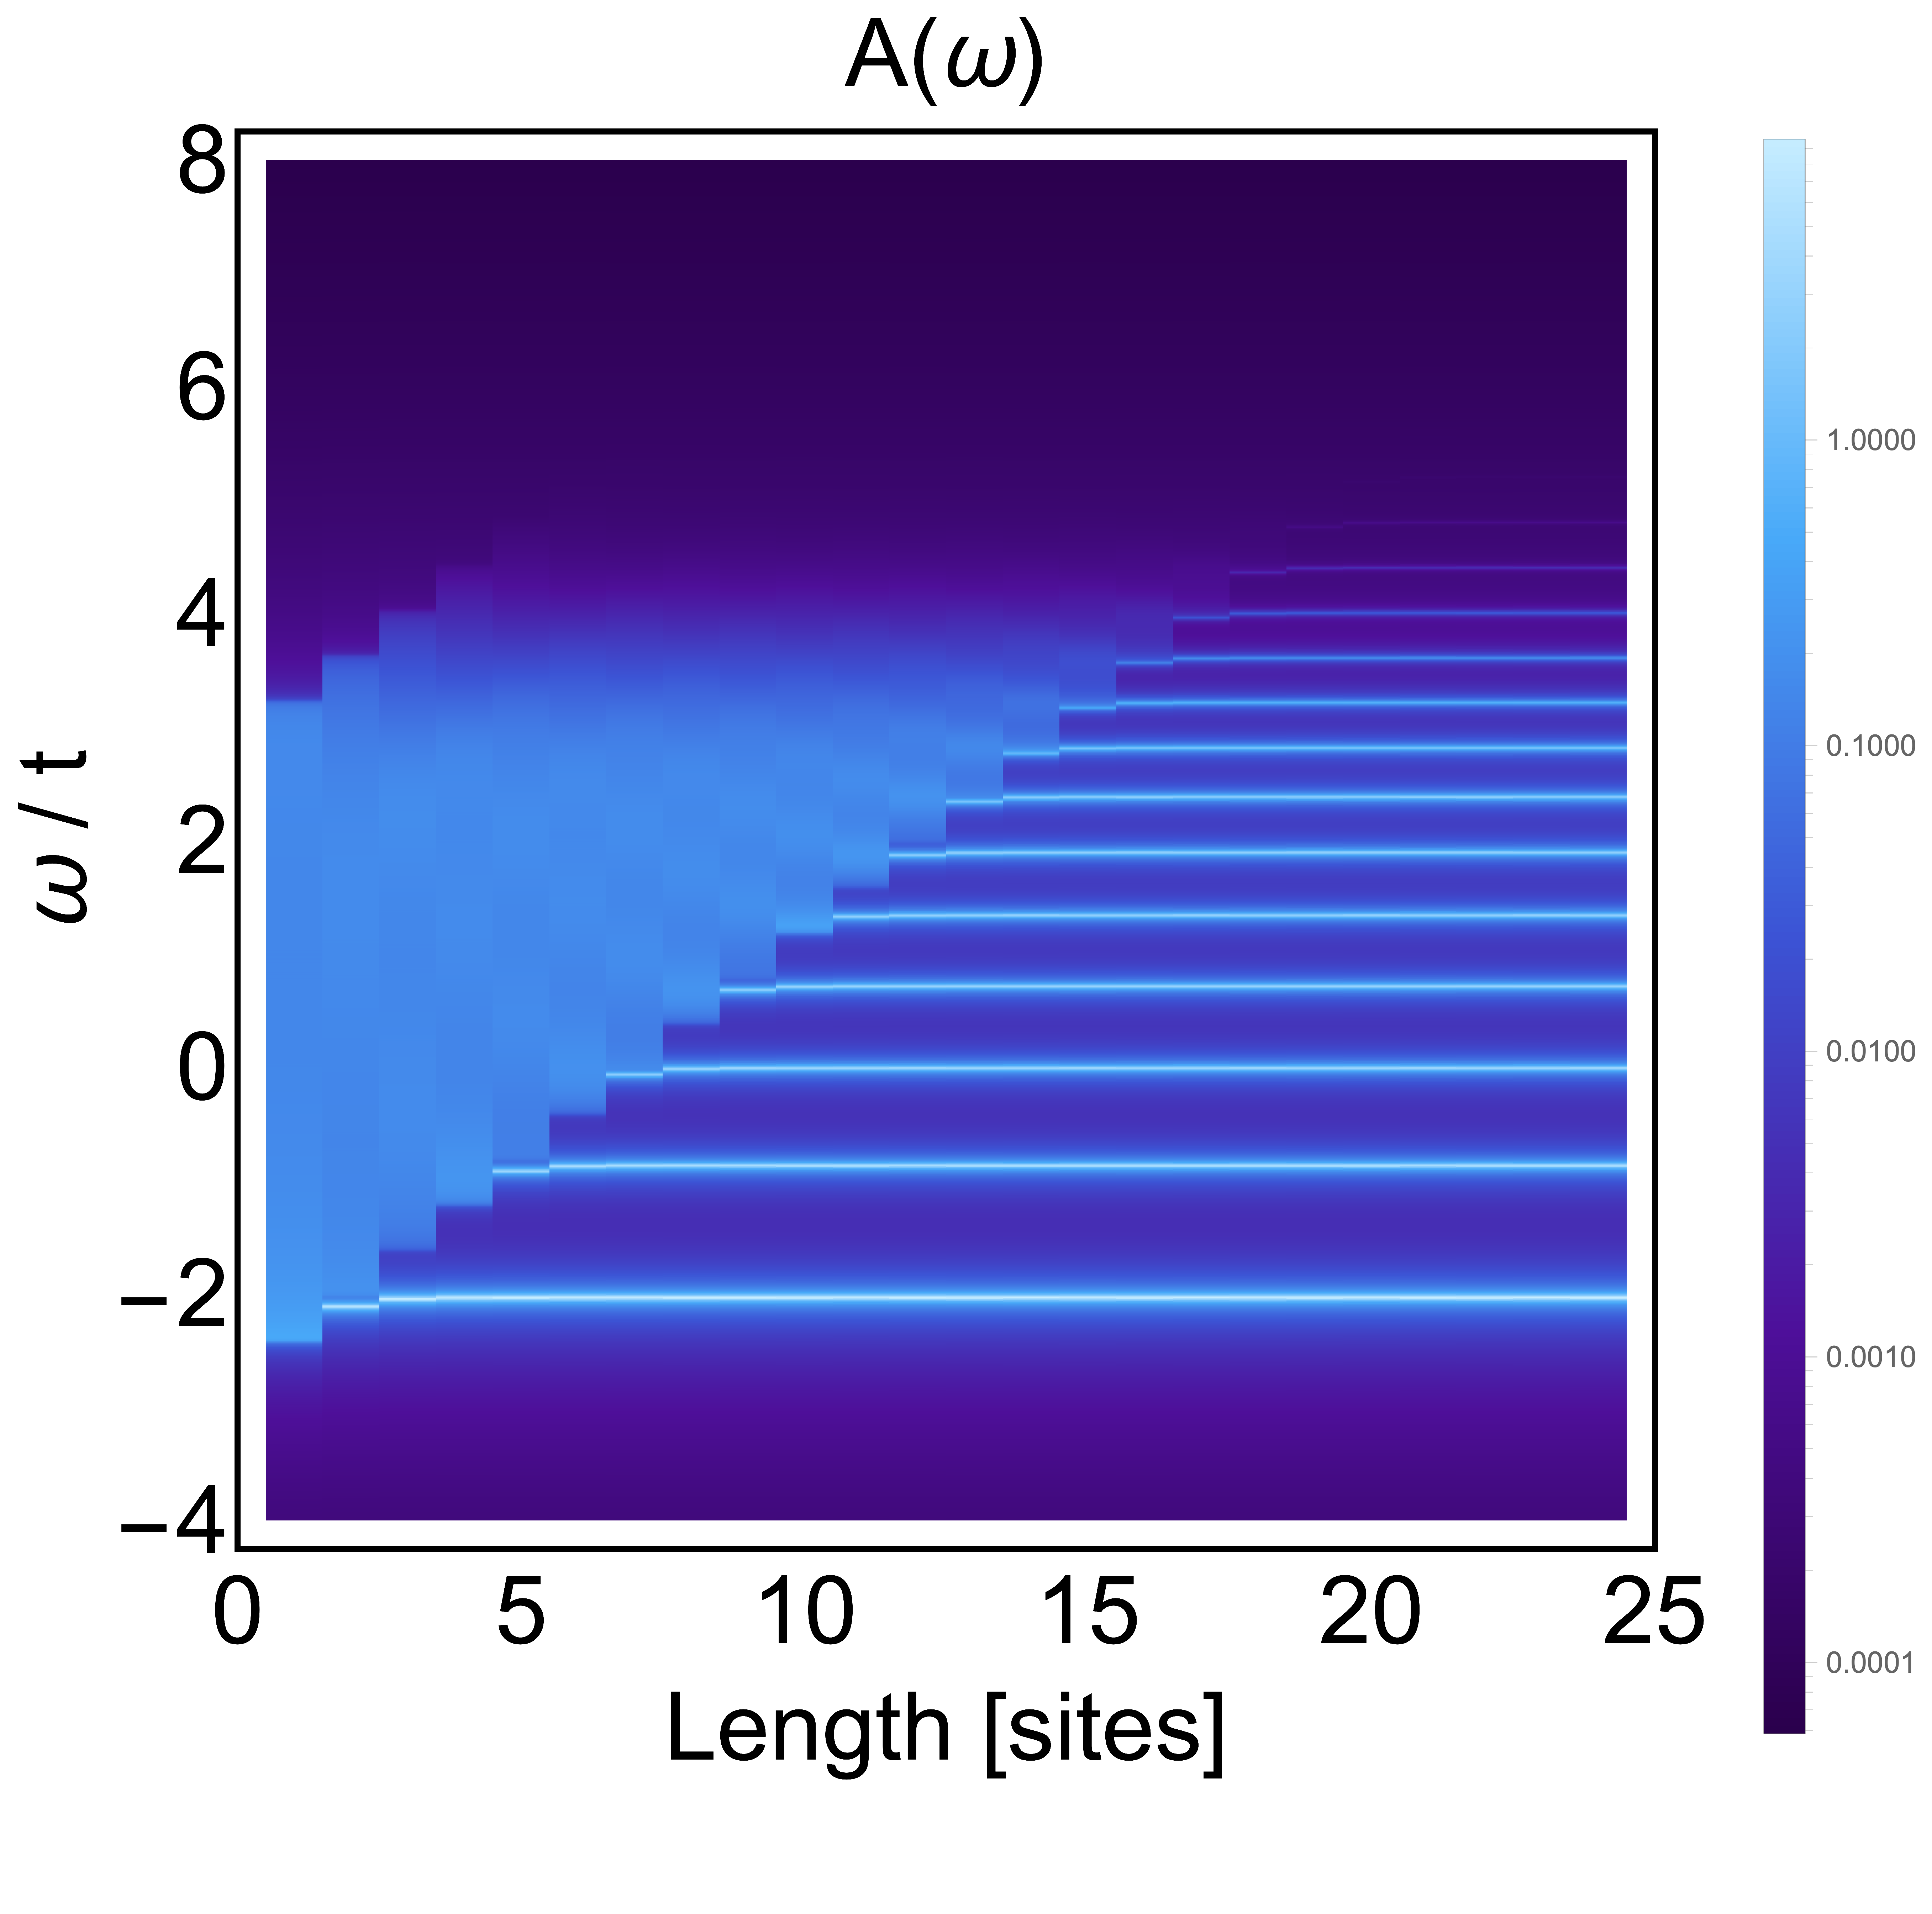
\includegraphics[width=0.4\textwidth]{Stepconst}
    \caption{Spectral function of a single hole for constant potential step $J = 0.4t$. Coordination number $z = 3$. Transition from continuum into a multiple QPs is observed resulting in $t\text{-}J^z$~model solution on the Bethe lattice.}\label{stepconst}
\end{figure}

\subsection{Discussion}
In Figs. \ref{areaconst}, \ref{V0const} and, \ref{stepconst}, spectrum at length of the well $L = 1$ corresponds to vertical cross of the density map of the point potential case (Fig. \ref{pointpotential}). It is visible that dependent on the point potential depth the solution may or may not contain the quasiparticle initially. Regardless of whether QP initially exists or not in all three cases (i), (ii) and, (iv) multiple peaks eventually appear when the width of the well grows. 

The range of energies where the quasiparticle solutions may exist corresponds to the depth of the potential well. For energies exceeding depth of the well potential there is always a continuum of states provided that well is not deeper than energy range covered by the continuum. This can be best visible in Fig. \ref{V0const} of case (ii) where the depth of the well is constant, $V_0 = 2t$. Of course, for small widths of the well the ground state is not at the bottom so the range of energies that is covered by QP solutions seems smaller then actual depth of the well. In cases (i) and (ii), when the width of the well is rising more and more solutions fit in the well while distances between them get smaller and smaller. In the thermodynamic limit when the well totally disappears the continuum rebuilds. In case (iv) in thermodynamic limit the linear potential covers whole lattice, thus one reproduces known $t\text{-}J^z$~model solution.

The case (iii) is different from others in that sense that it is the only case where the width of the well is constant. The vertical cross of Fig. \ref{widthconst} at $V_0 = LJ = 4.8t$ is equal to the vertical cross through Fig. \ref{stepconst} at length $L = 12$ (where $J = 0.4t$).


\end{document}

